\documentclass[11pt,a4paper]{article}
\usepackage{fontspec}
\setmainfont{TeX Gyre Pagella}
\newfontfamily\headfont{Inter}[UprightFont=*-ExtraBold,BoldFont=*-ExtraBold,Extension=.otf,Path=/usr/share/fonts/opentype/inter/]
\usepackage[a4paper,margin=2.3cm]{geometry}
\usepackage{graphicx,booktabs,float,caption,array,xcolor,longtable}
\usepackage{xurl}
\usepackage[hidelinks]{hyperref}
\usepackage{titlesec}
\usepackage[round]{natbib}
\usepackage{setspace}
\setstretch{1.05}
\renewcommand{\topfraction}{0.9}
\renewcommand{\bottomfraction}{0.8}
\renewcommand{\textfraction}{0.1}
\renewcommand{\floatpagefraction}{0.75}
\setlength{\parindent}{0pt}
\setlength{\parskip}{0.55em}
\titleformat{\section}{\headfont\Large}{\thesection}{0.8em}{}
\titleformat{\subsection}{\headfont\large}{\thesubsection}{0.8em}{}
\captionsetup{font=small,labelfont=bf}
\urlstyle{same}
\hypersetup{pdftitle={Where Football Clubs Come From},pdfauthor={Tristan Hotham}}

\begin{document}
\begin{center}
{\Large\bfseries Where Football Clubs Come From\par}
\vspace{0.4em}
{\large Founding years of 45,931 association football clubs in Wikidata,\\from Sheffield FC in 1857 to today\par}
\vspace{1.2em}
{\large Tristan Hotham\par}
\vspace{0.3em}
{\small Independent researcher\\
ORCID: 0000-0003-4931-9349\\
DOI: \href{https://doi.org/10.5281/zenodo.23844505}{https://doi.org/10.5281/zenodo.23844505}\par}
\vspace{0.8em}
2026
\end{center}

\begin{quote}
\small
\begin{center}\textbf{Abstract}\end{center}
Association football spread from a handful of clubs in northern England in the 1850s and 1860s to almost every country on earth. I use Wikidata, the open knowledge base behind Wikipedia, to map that spread from the bottom up: every item that is an association football club, with its founding year, its dissolution year and a location. After removing national teams, reserve and youth sides, beach soccer and futsal teams and probable Australian rules clubs, 45,931 clubs remain, 27,079 (59\%) with a founding year and 16,227 (35\%) with a point. The oldest dated club Wikidata records in each of 222 countries and territories traces a diffusion front: 55 had a club before 1900 and 173 before 1950, and first clubs founded before 1900 lie a median 1,966 km from Sheffield against 6,894 km for those founded after 1950. Before 1900, 93\% of new clubs were European and 59\% were in the United Kingdom; the busiest year is 1919 (475 clubs), Europe's busiest decade the 1920s, and every other continent's the 2000s. Wikidata records 4,091 dissolutions, peaking in 1945 (174 clubs, 143 of them German). Coverage is very uneven: the Netherlands has 165 clubs per million people in Wikidata and Nigeria 0.6. The atlas maps what the open record says about where clubs come from, and is explicit about what it cannot say, including who founded them.

\textbf{Keywords:} football; soccer; association football clubs; diffusion; sport history; Wikidata; open data; mapping
\end{quote}

\section{Introduction}
Sheffield FC, founded in 1857, is usually called the oldest football club in the world, and the game that the Football Association codified in London in 1863 spread with remarkable speed. Historians have told that story through rules, associations and individual pioneers: public school and working-class football in England \citep{harvey}, and the global spread carried by trade, empire, migration and education \citep{goldblatt,giulianotti}. What is harder to see is the aggregate pattern, the thousands of clubs founded decade after decade, country after country.

Wikidata \citep{wikidata} offers a way to look at that pattern from the bottom up. It is an open, structured database of named things, including tens of thousands of football clubs, many with a founding date, a location or a home ground, and some with a dissolution date. It is also uneven, catalogued by volunteers with very different interests in different countries. This paper uses it to ask three simple questions: when did each country get its first (recorded) club, how did club founding rise and fall by decade and continent, and which clubs did not survive? It pairs the analysis with an interactive, animated atlas (\url{https://maps.tristanhotham.com/football-origins/}).

The contribution is descriptive and deliberately modest. Wikidata is not a census of clubs, and a founding year in Wikidata is not proof of when football was first played anywhere. I am explicit throughout about coverage, and about one question the data cannot answer: who founded these clubs. Wikidata does not record the nationality of founders, so nothing here measures the part played by British workers, sailors, engineers or students abroad, however prominent it is in the literature.

\section{Data}
\textbf{Wikidata.} A single query through the QLever SPARQL endpoint \citep{qlever}, retrieved in 2026, returned every item that is an instance of association football club (Q476028) or of one of its subclasses, with its English label, inception (P571), dissolution (P576), coordinates (P625), the coordinates of its home venue (P115), country (P17), number of sitelinks and class. Because each combination of these values is a row, the result has 48,286 rows for 46,993 items. Wikidata is published under CC0.

\textbf{Geography.} Natural Earth \citep{naturalearth} countries (1:50m for display, 1:10m for point in polygon), states and provinces (to split the United Kingdom into England, Scotland, Wales and Northern Ireland, each of which has its own football association), populated places (for clubs whose name contains a town) and population estimates. All are public domain.

\textbf{Check.} The engsoccerdata club table \citep{engsoccer} gives coordinates for 465 English clubs that match Wikidata labels; 451 of them lie within 10 km of the Wikidata point. The two sources are probably not independent (both draw on Wikipedia), so this checks transcription rather than truth.

\begin{table}[tbp]\centering\small\caption{From query to data.}\label{tab:pipe}\begin{tabular}{p{9.5cm}r}\toprule Step & Items\\\midrule
Rows returned by the query & 48,286\\
Distinct Wikidata items & 46,993\\
Left out: national teams, beach and futsal, reserve and youth teams, Australian rules clubs & 1,062\\
Clubs kept & 45,931\\
\quad with a founding year & 27,079\\
\quad\quad of which from 1857 (used for the timeline) & 27,059\\
\quad with a point (own 3,004; ground 10,046; town in name 3,177) & 16,227\\
\quad with a founding year from 1857 and a point (on the animated map) & 12,589\\
\quad with a present-day country & 42,032\\
\quad with a dissolution year & 4,097\\
\bottomrule\end{tabular}\end{table}

\section{Methods}
\subsection{Which items are clubs}
I kept one record per item and pooled values across rows. I left out 1,062 items that are not clubs in the usual sense: 377 national and representative teams (by class or by names such as `national football team'), 88 beach soccer and futsal sides, 428 reserve, B, II and under-age teams (which repeat the founding year of their parent club), and 169 Australian clubs whose names (a spelt-out `Football Club', `Football Netball Club' or `Australian Football Club' with no soccer word) mark them as Australian rules football clubs, a class Wikidata often confuses with association football. These filters are name based and imperfect in both directions.

\subsection{Dates}
The founding year is the earliest inception year of an item; 86\% of founding dates are stored as 1 January, which in Wikidata usually means that only the year is known, so I work in years throughout. 20 clubs have a founding year before 1857. On inspection these are cricket, rowing, gymnastics and multi-sport societies older than the football they later took up, plus a few errors (a Spanish club dated 1492, an Ecuadorian club dated a century early); they are kept in the data with a flag but left out of the timeline and the first-club analysis. One founding year in the future (1 club) was removed. The dissolution year is the latest P576 year; 6 clubs with a dissolution before their founding are flagged and left out of the dissolution counts.

\subsection{Places and countries}
A club's point is its own coordinates (3,004 clubs), else its home venue's (10,046), else, if its English label contains the name of a Natural Earth populated place in the same country (excluding common words such as Union, Victoria or Santa), that place (3,177). The last is approximate and is flagged. A club's country is the present-day country (or UK nation) that its point falls in, else the country Wikidata gives, matched to Natural Earth by Wikidata identifier. Where both are known they agree for 98\% of 12,796 clubs. 457 clubs whose only country is a former state (the Soviet Union, the German Reich, Czechoslovakia, Austria-Hungary, Yugoslavia) and that have no point are kept in the totals but given no present-day country, and 1,489 UK clubs with no point stay as `United Kingdom'. Continents follow Natural Earth, with small island states assigned to their nearest continent.

\subsection{First clubs and the diffusion front}
For each country I take the oldest club with a founding year from 1857 (ties broken by sitelinks), and measure the great-circle distance from Sheffield to its point (or to the country's label point if it has none). I use this as a simple, transparent diffusion front, not as a model of diffusion: it tells us when a club that still has a Wikidata entry was founded, which may be long after football was first played, and in multi-sport societies may be long before.

\section{Results}
\subsection{The spread}
Figure~\ref{fig:snap} shows every dated club with a point at six moments. In 1870, 61\% of the 84 clubs in the record are in the United Kingdom, with outliers in a handful of other countries, several of them older sports societies; by 1890 they cover the British Isles densely and are scattered through the ports and cities of western Europe, the River Plate, India, southern Africa and Australia; by 1930 they cover Europe and much of South America; after 1960 they reach almost everywhere. By 2026 the record holds 222 countries and territories with a dated club.

\begin{figure}[tbp]\centering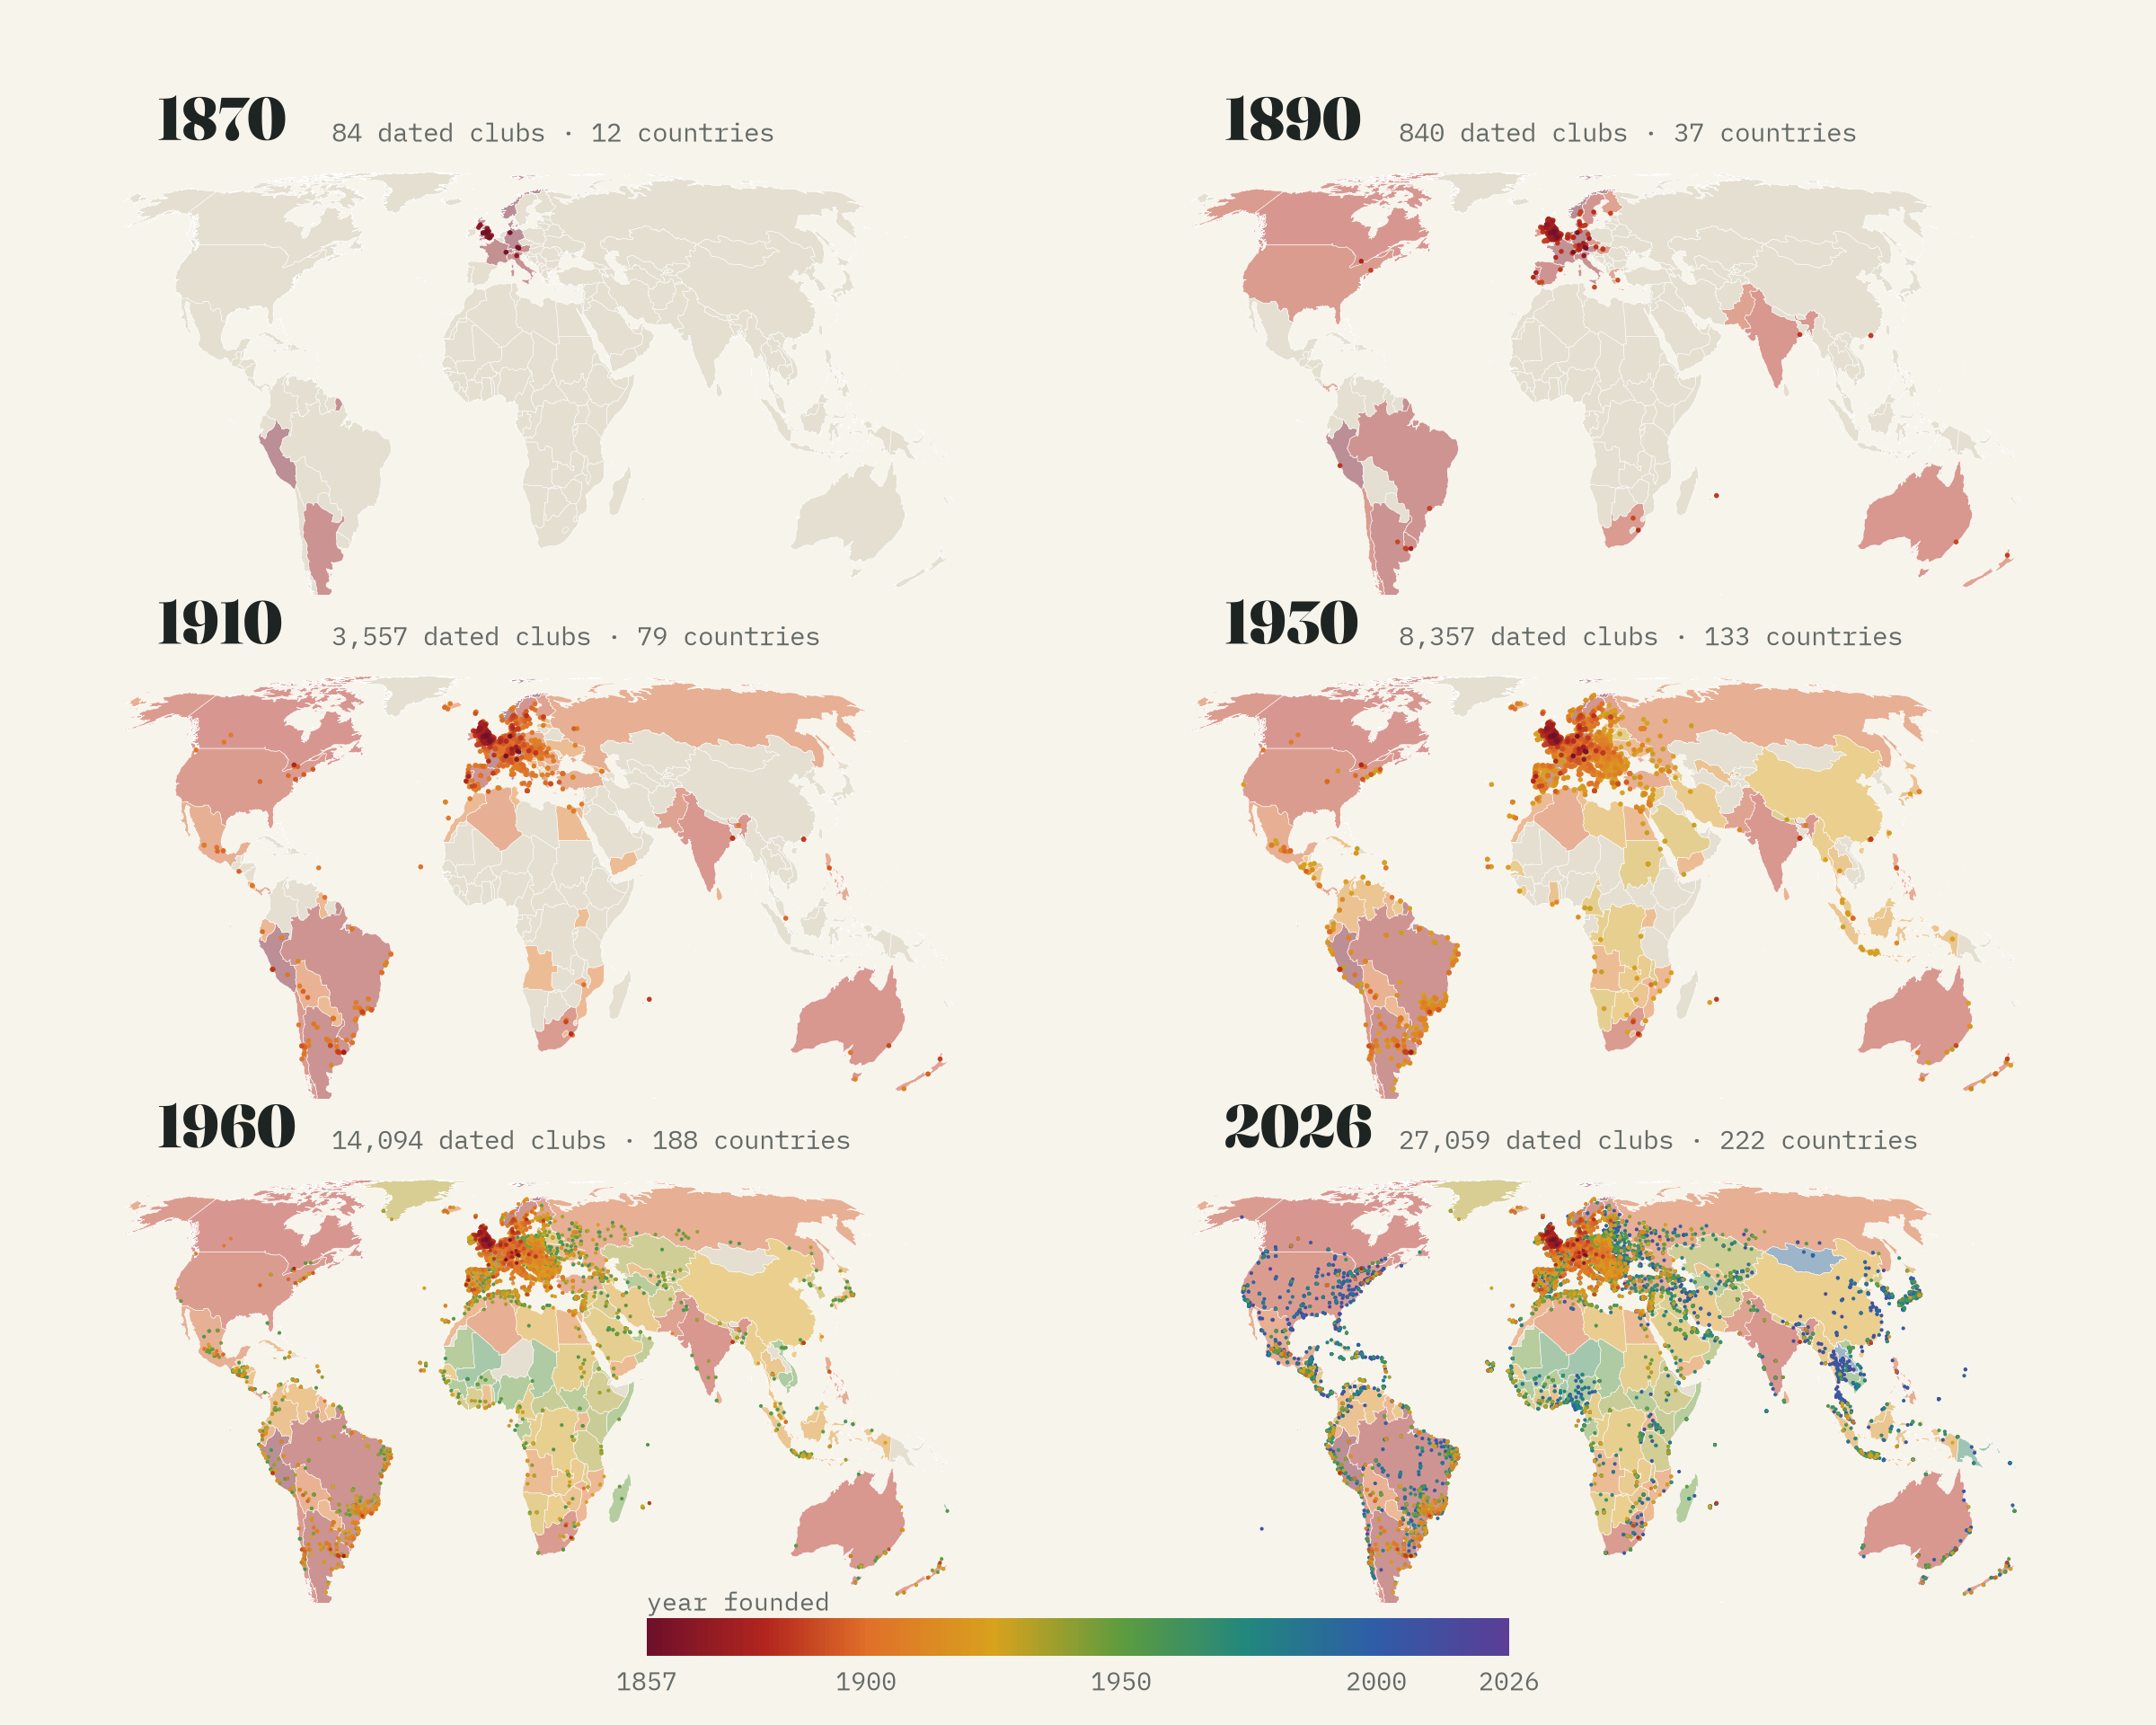
\includegraphics[width=\textwidth]{f_snapshots.png}
\caption{Clubs with a founding year and a point, by year founded, at six moments. Countries are shaded once they have a dated club.}\label{fig:snap}\end{figure}

\subsection{First clubs}
Figure~\ref{fig:first} maps the year of each country's oldest dated club, and Figure~\ref{fig:front} plots it against distance from Sheffield. The pattern is a front that moves outwards but leaps by sea. Countries whose first club came before 1900 sit a median 1,966 km from Sheffield, those after 1950 a median 6,894 km, and the correlation between year and distance is a modest 0.36. Peru (the Lima Cricket and Football Club, 1859), Argentina, Uruguay, India and Australia all have clubs in the record before Hungary, Poland or Russia. Table~\ref{tab:cont} summarises by continent and Table~\ref{tab:first} lists the earliest first clubs.

Many first clubs are multi-sport societies. Switzerland's is the Lausanne Football and Cricket Club (1860), Uruguay's the Montevideo Rowing Club (1874), Norway's a gymnastics society in Drammen (1857), Italy's the Bentegodi gymnastics society in Verona (1868). Wikidata records the founding of the whole club, so these dates say when a club that now has a football side was founded. Others are surprising and may be wrong: France's oldest dated club, a club in Cergy-Pontoise, is given 1865.

\begin{figure}[tbp]\centering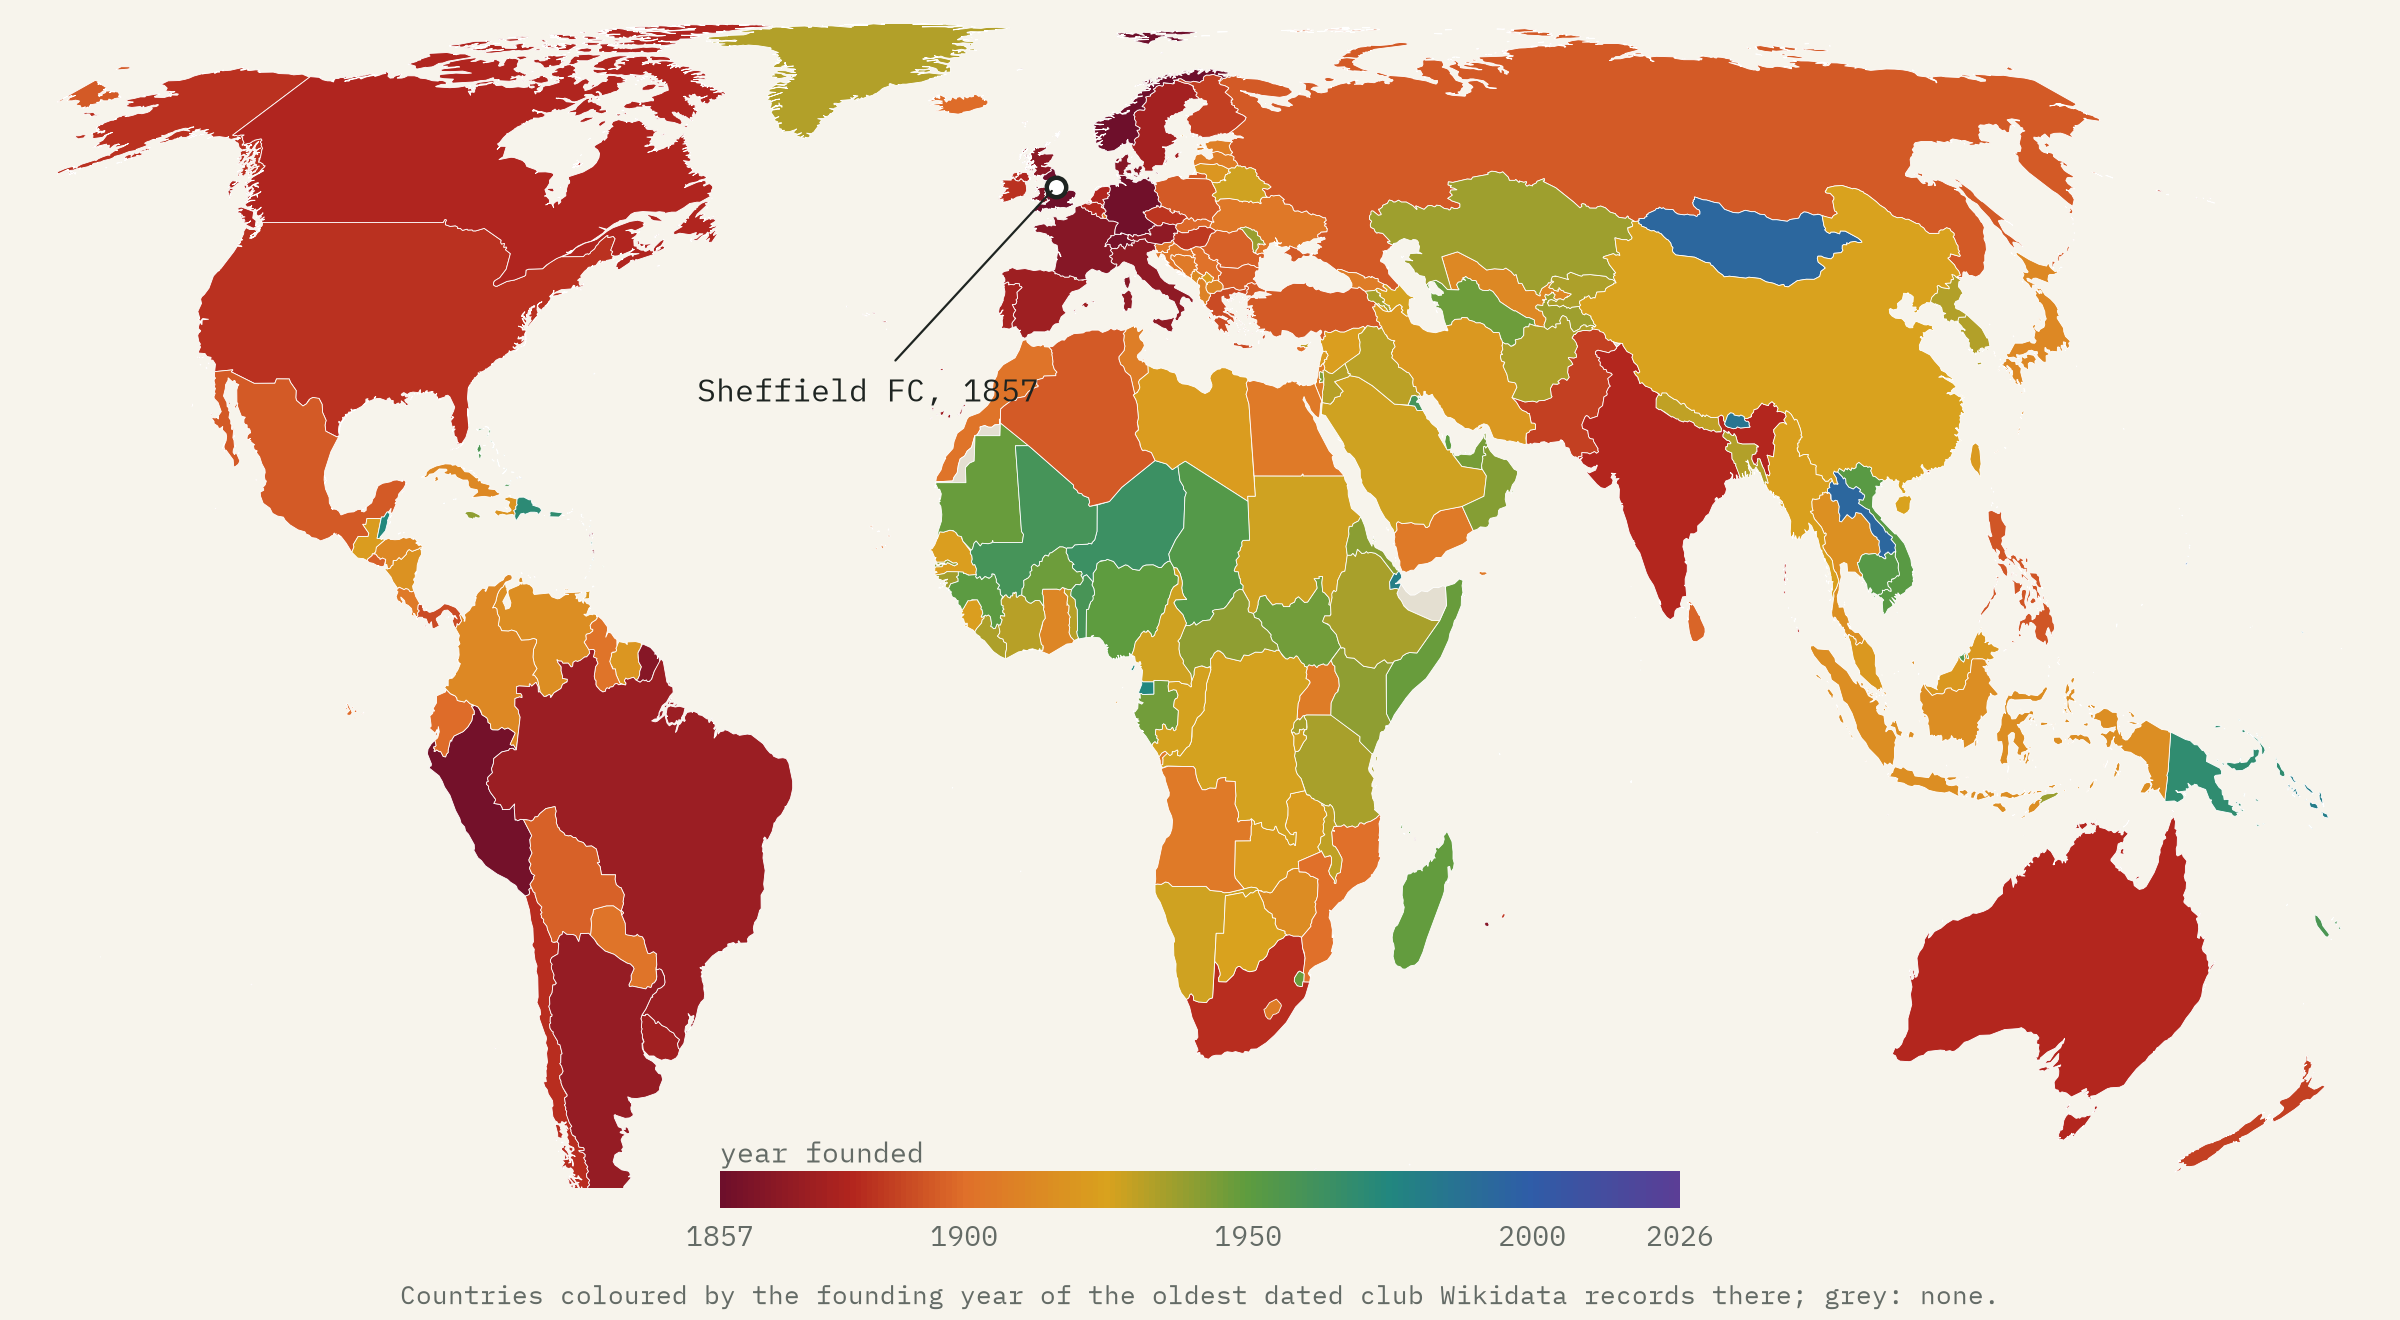
\includegraphics[width=\textwidth]{f_first_map.png}
\caption{Year of the oldest dated club in Wikidata, by country.}\label{fig:first}\end{figure}

\begin{figure}[tbp]\centering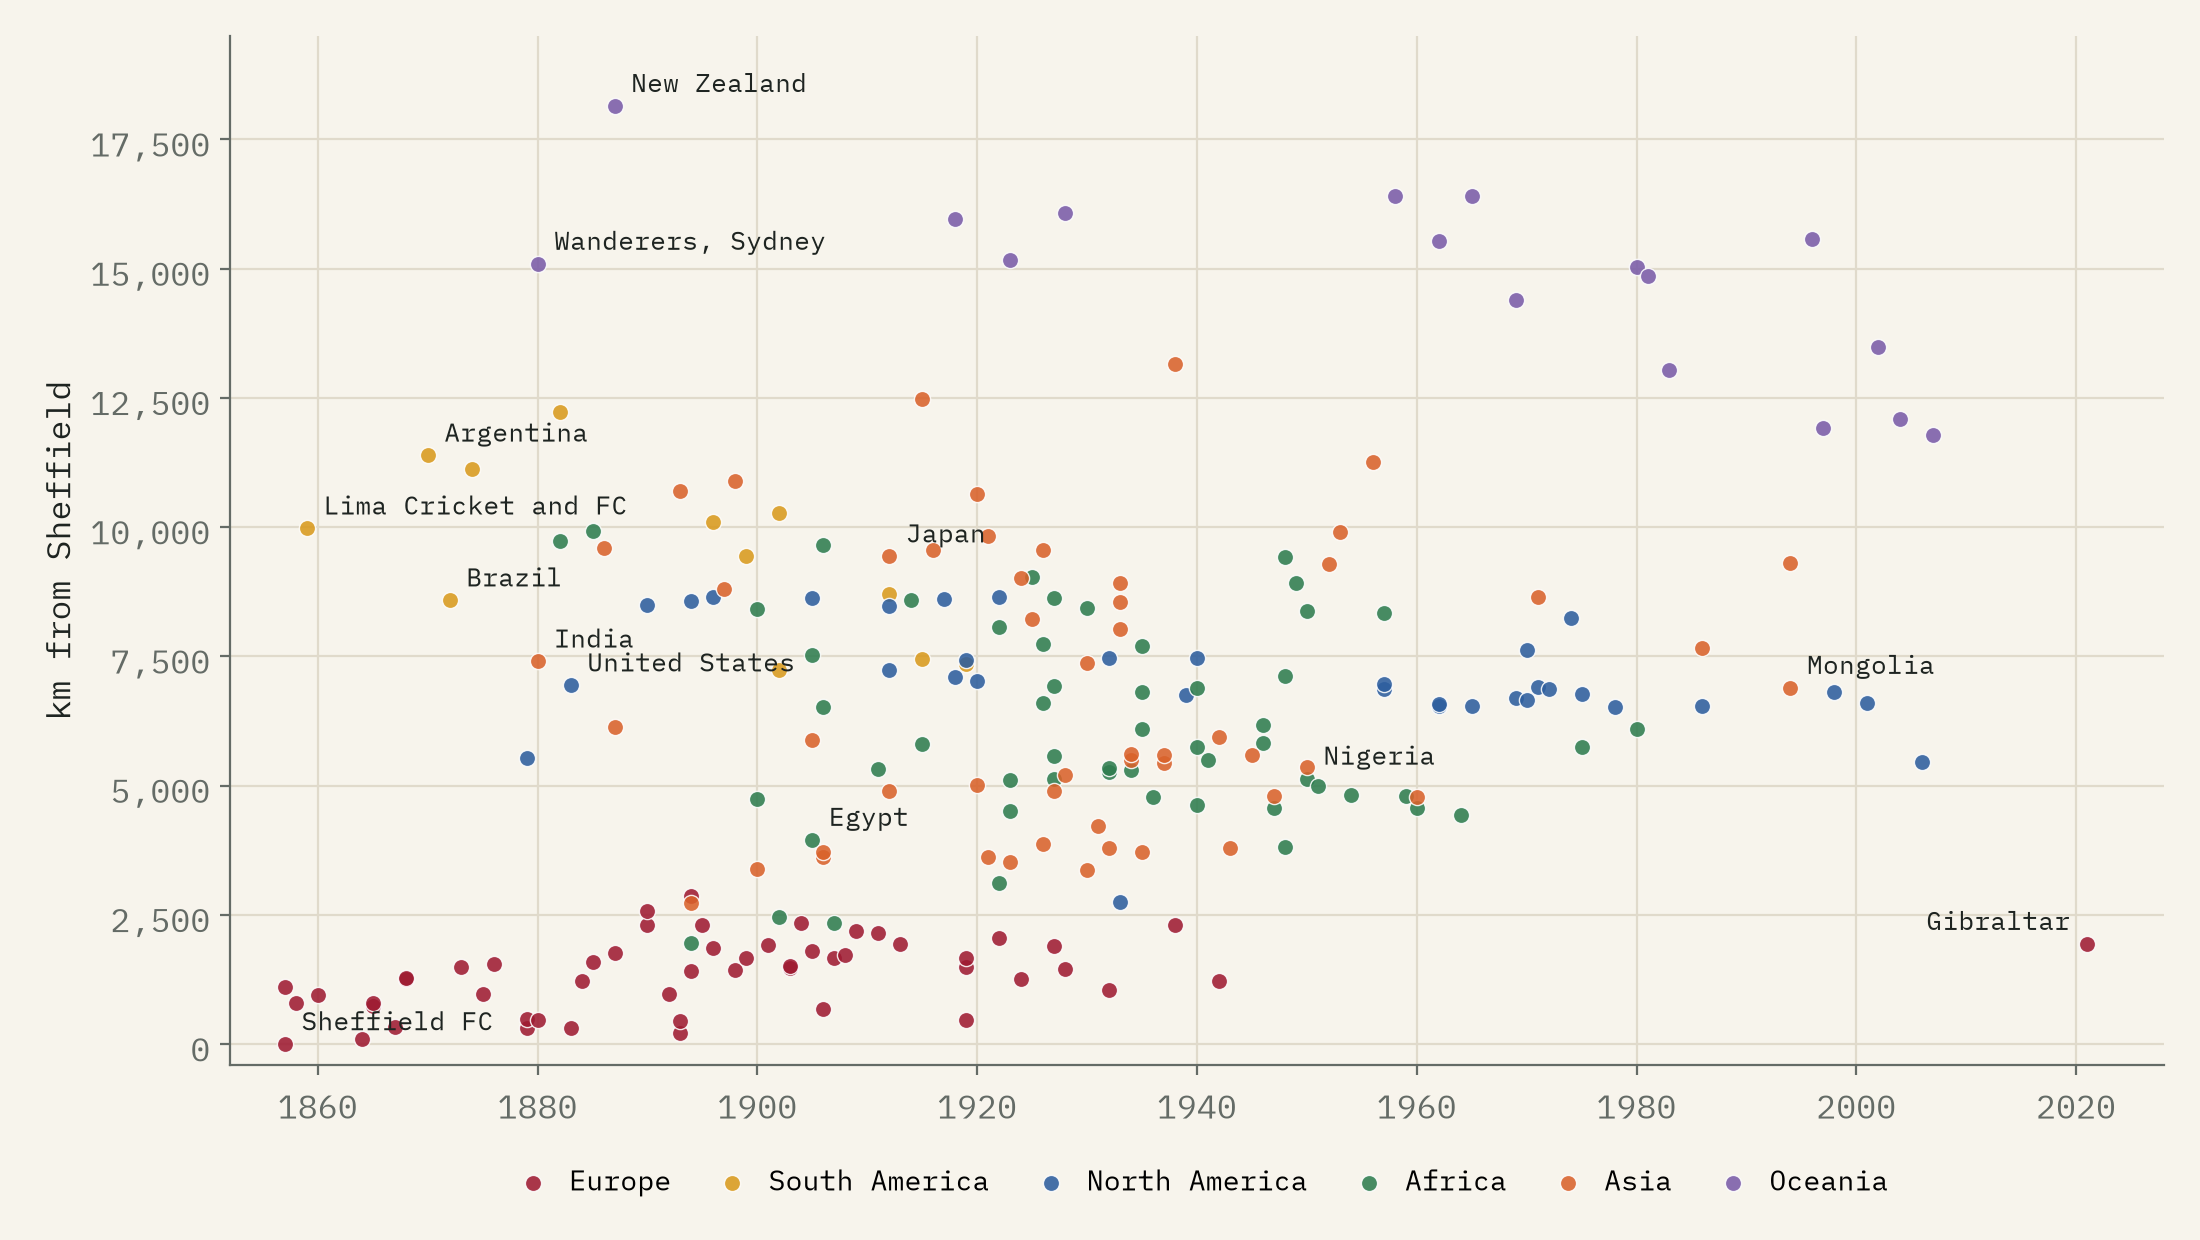
\includegraphics[width=.95\textwidth]{f_front.png}
\caption{The diffusion front: year of each country's oldest dated club against the distance of that club from Sheffield.}\label{fig:front}\end{figure}

\begin{table}[tbp]\centering\small\caption{First clubs by continent: number of countries and territories with a dated club, the earliest, and the median year of countries' first clubs.}\label{tab:cont}\setlength{\tabcolsep}{4pt}\begin{tabular}{lr>{\raggedright\arraybackslash}p{2.6cm}>{\raggedright\arraybackslash}p{4.8cm}rr}\toprule Continent & Countries & Earliest & Club & Year & Median\\\midrule
Europe & 53 & England & Sheffield F.C. & 1857 & 1894\\
South America & 12 & Peru & Lima Cricket and Football Club & 1859 & 1898\\
North America & 34 & Canada & Toronto Varsity Blues men's soccer & 1879 & 1948\\
Africa & 54 & South Africa & Savages FC Pietermaritzburg & 1882 & 1932\\
Asia & 52 & India & Dalhousie AC & 1880 & 1929\\
Oceania & 17 & Australia & Wanderers F.C. & 1880 & 1969\\
\bottomrule\end{tabular}\end{table}

\begin{table}[tbp]\centering\footnotesize\caption{The earliest first clubs: the oldest dated club Wikidata records in each country or territory, first 36 (all are in data/first\_clubs.csv).}\label{tab:first}\begin{tabular}{rl>{\raggedright\arraybackslash}p{7.2cm}r}\toprule Year & Country & Club & km from Sheffield\\\midrule
1857 & England & Sheffield F.C. & 3\\
1857 & Norway & Drammens TF & 1,108\\
1858 & Germany & SV 1858 Alfeld/Leine & 805\\
1859 & Peru & Lima Cricket and Football Club & 9,977\\
1860 & Switzerland & Lausanne Football and Cricket Club & 957\\
1864 & Wales & Wrexham A.F.C. & 109\\
1865 & Denmark & Skamby Boldklub & 732\\
1865 & France & Cergy Pontoise FC & 796\\
1867 & Scotland & Queen's Park F.C. & 326\\
1868 & Italy & Bentegodi Verona & 1,258\\
1868 & Austria & (no English label) Q63306374 & 1,278\\
1870 & Argentina & Club Atlético Carcarañá & 11,387\\
1872 & Brazil & Paissandu Atlético Clube & 8,586\\
1873 & Spain & Exiles Cable Club & 1,486\\
1874 & Uruguay & Montevideo Rowing Club & 11,134\\
1875 & Sweden & Göteborgs BK & 970\\
1876 & Portugal & Associação Académica de Coimbra, O.A.F. & 1,556\\
1879 & Northern Ireland & Cliftonville F.C. & 324\\
1879 & Netherlands & Koninklijke HFC & 486\\
1879 & Canada & Toronto Varsity Blues men's soccer & 5,545\\
1880 & Belgium & Royal Antwerp F.C. & 469\\
1880 & India & Dalhousie AC & 7,404\\
1880 & Australia & Wanderers F.C. & 15,096\\
1882 & South Africa & Savages FC Pietermaritzburg & 9,728\\
1882 & Chile & (no English label) Q5988624 & 12,231\\
1883 & Ireland & Dublin University Association Football Club & 318\\
1883 & United States & Clark O.N.T. & 6,942\\
1884 & Czech Republic & FK Jiskra Třeboň & 1,223\\
1885 & Hungary & Újpest FC & 1,584\\
1885 & Mauritius & Arsenal Wanderers & 9,928\\
1886 & Hong Kong & HKFC Soccer Section & 9,591\\
1887 & Finland & Helsingin Ponnistus & 1,761\\
1887 & Pakistan & KPT F.C. & 6,137\\
1887 & New Zealand & North Shore United AFC & 18,148\\
1890 & Malta & St. George's F.C. & 2,304\\
1890 & Greece & Panionios F.C. & 2,578\\
\bottomrule\end{tabular}\end{table}

\subsection{The British Isles}
Of the 314 clubs dated before 1880, 258 are in the United Kingdom (Figure~\ref{fig:uk}). The first club in each nation is Sheffield FC in England (1857), Wrexham in Wales (1864), Queen's Park in Scotland (1867) and Cliftonville in Northern Ireland (1879). England's early list includes Hallam (1860), Notts County (1862), Stoke (1863), Nottingham Forest (1865) and Sheffield Wednesday (1867), and London clubs of the early FA Cup, such as the Wanderers, that no longer exist.

\begin{figure}[tbp]\centering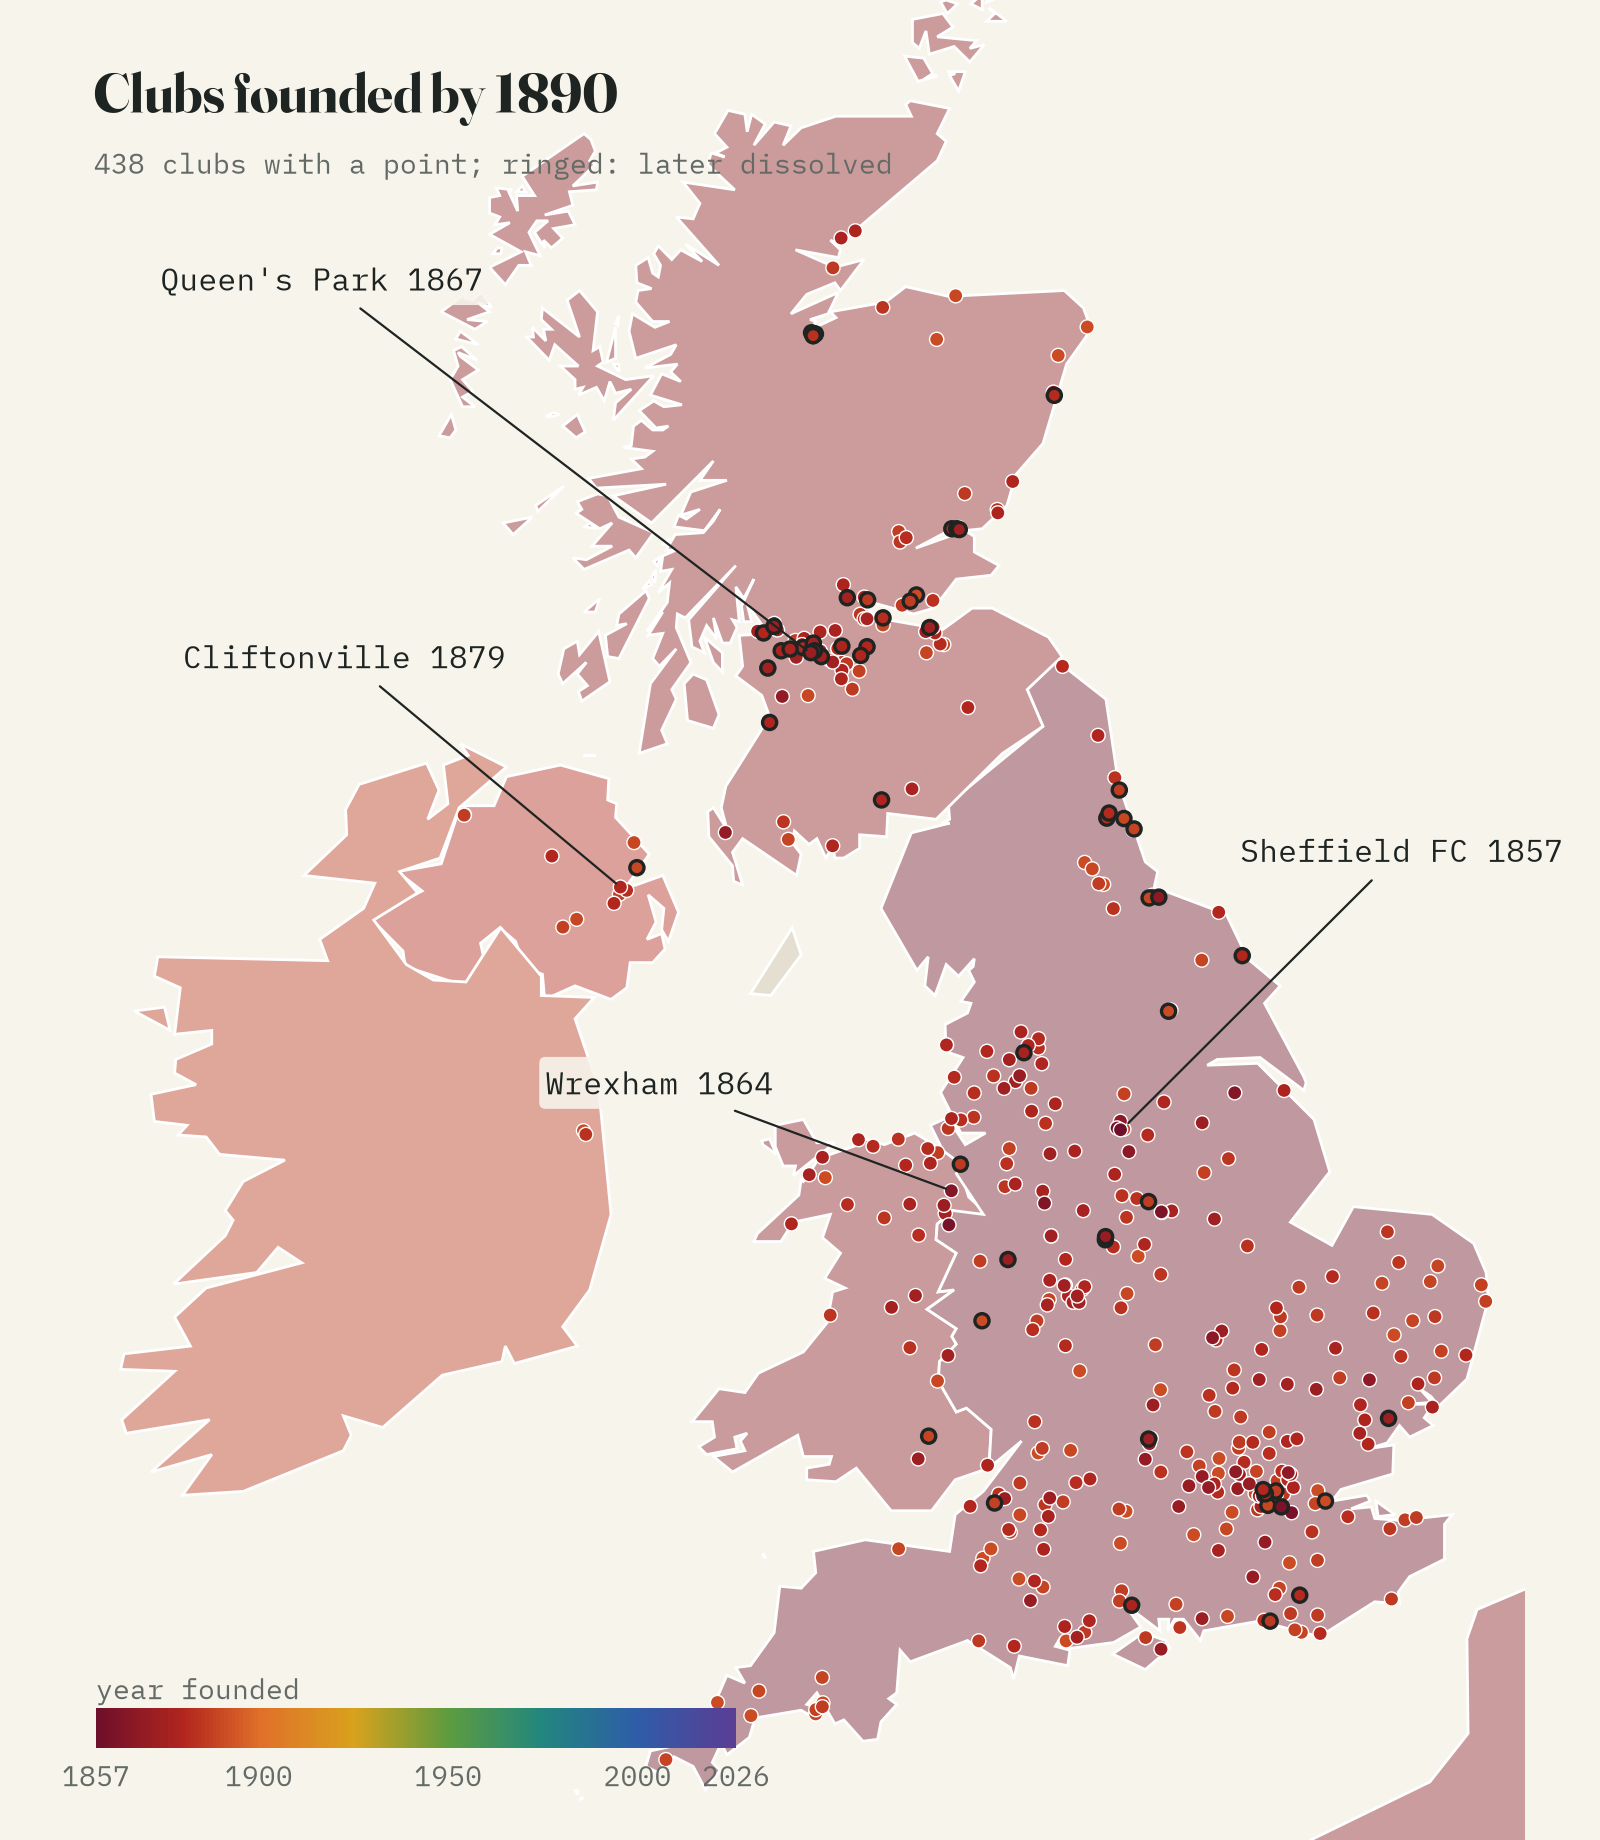
\includegraphics[width=.72\textwidth]{f_british_isles.png}
\caption{Clubs in the British Isles founded by 1890, by year founded. Ringed: later dissolved.}\label{fig:uk}\end{figure}

\subsection{Founding waves}
Figure~\ref{fig:waves} shows clubs founded per decade by continent. Europe dominates the early record (93\% of clubs founded before 1900 and 79\% from 1900 to 1949) and peaks in the 1920s; the single busiest year is 1919 (475 clubs), as the First World War ended. Every other continent peaks in the 2000s, and since 2000 Europe's share of new clubs falls to 38\%, with Asia at 26\% and North America at 17\%. Clubs founded since 1990 make up 29\% of dated clubs. Part of the recent rise is real (new professional leagues, independent states, women's football) and part reflects recording: recent clubs are more likely to have a founding date and an entry at all.

\begin{figure}[tbp]\centering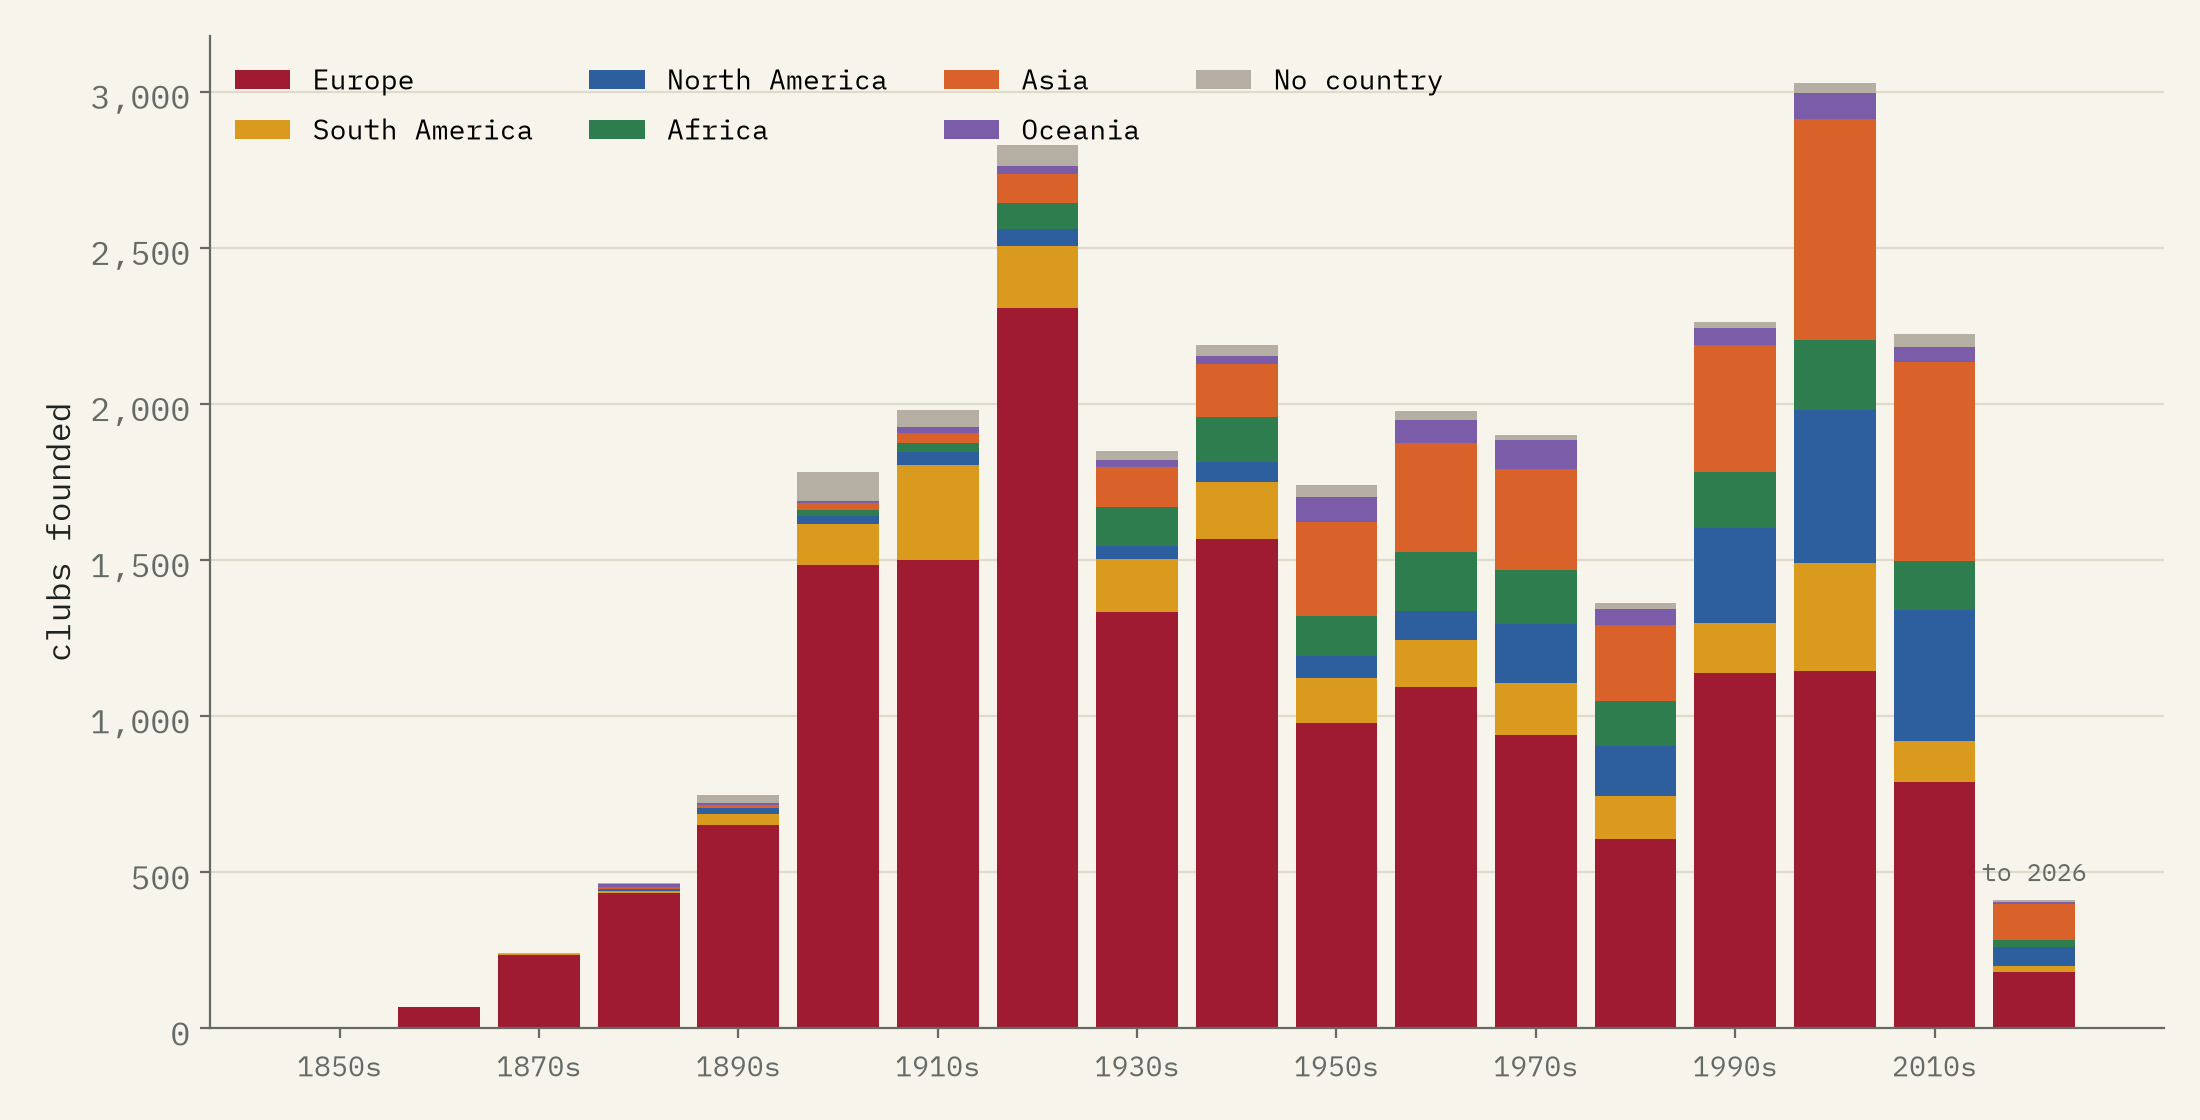
\includegraphics[width=\textwidth]{f_waves.png}
\caption{Clubs founded per decade, by continent (27,059 clubs with a founding year from 1857). The 2020s run to 2026.}\label{fig:waves}\end{figure}

\subsection{Clubs that died}
Wikidata records a dissolution for 4,091 clubs (9\%), shown by decade in Figure~\ref{fig:dis}. The single worst year is 1945: 174 clubs, 143 of them in Germany or with the German Reich as their country, when the Allied Control Council dissolved German sports organisations and clubs in the lost eastern territories ceased to exist. Since 2000 there have been 2,144 recorded dissolutions (52\% of the total), a mixture of real closures, mergers and refoundings and of easier recording. Among clubs with both dates the median lifespan is 23 years, and 791 lasted five years or fewer. The oldest club recorded as dissolved is the Wanderers (1859 to 1887).

\begin{figure}[tbp]\centering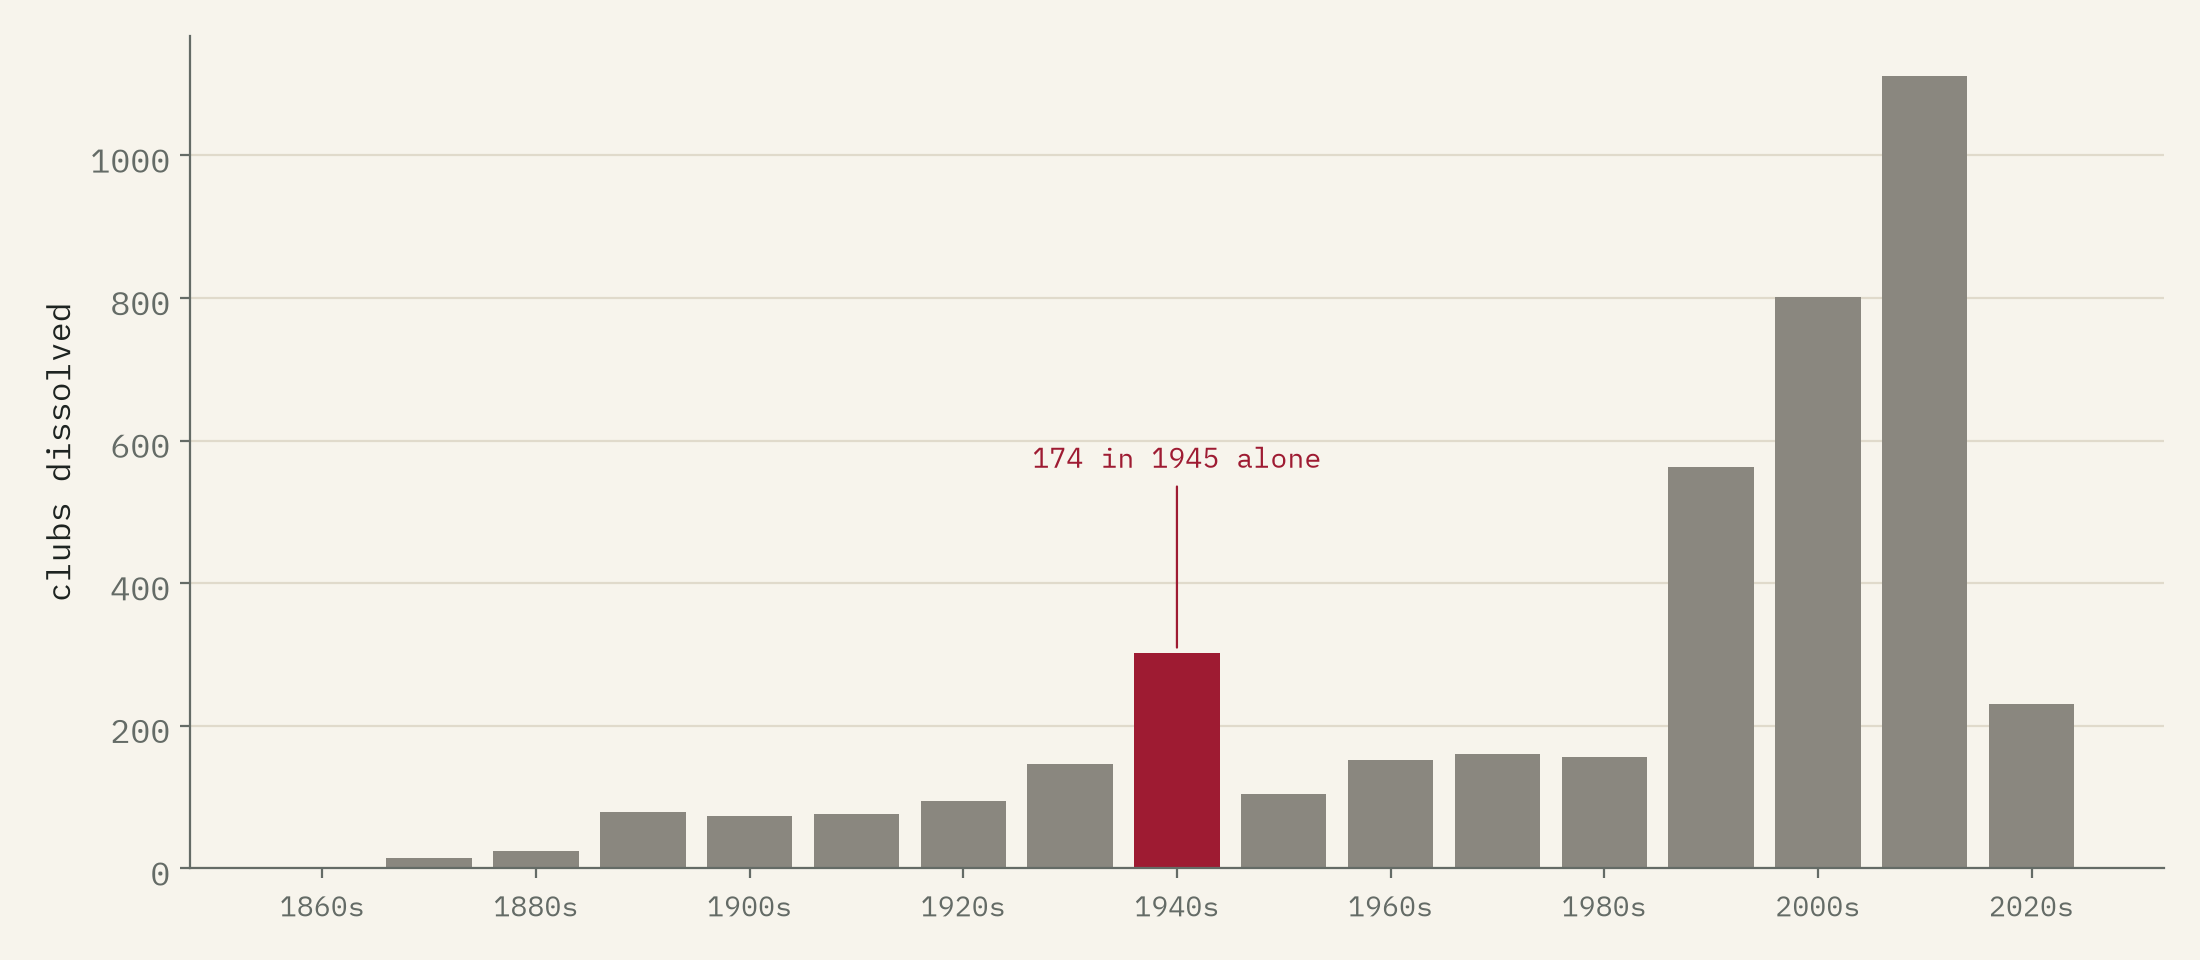
\includegraphics[width=.95\textwidth]{f_dissolved.png}
\caption{Clubs dissolved per decade (P576).}\label{fig:dis}\end{figure}

\subsection{Coverage}
Europe holds 61\% of clubs with a country, Asia 14\% and Africa 8\% (Table~\ref{tab:cov}). Per head of population, Wikidata has 165 clubs per million people in the Netherlands and 0.6 in Nigeria (Figure~\ref{fig:cov}); the most catalogued countries per head are small European ones where editors have entered amateur and village clubs systematically. Clubs are thinly described: half have 2 or fewer sitelinks and 44\% at most one, and 11,733 have no English label.

\begin{figure}[tbp]\centering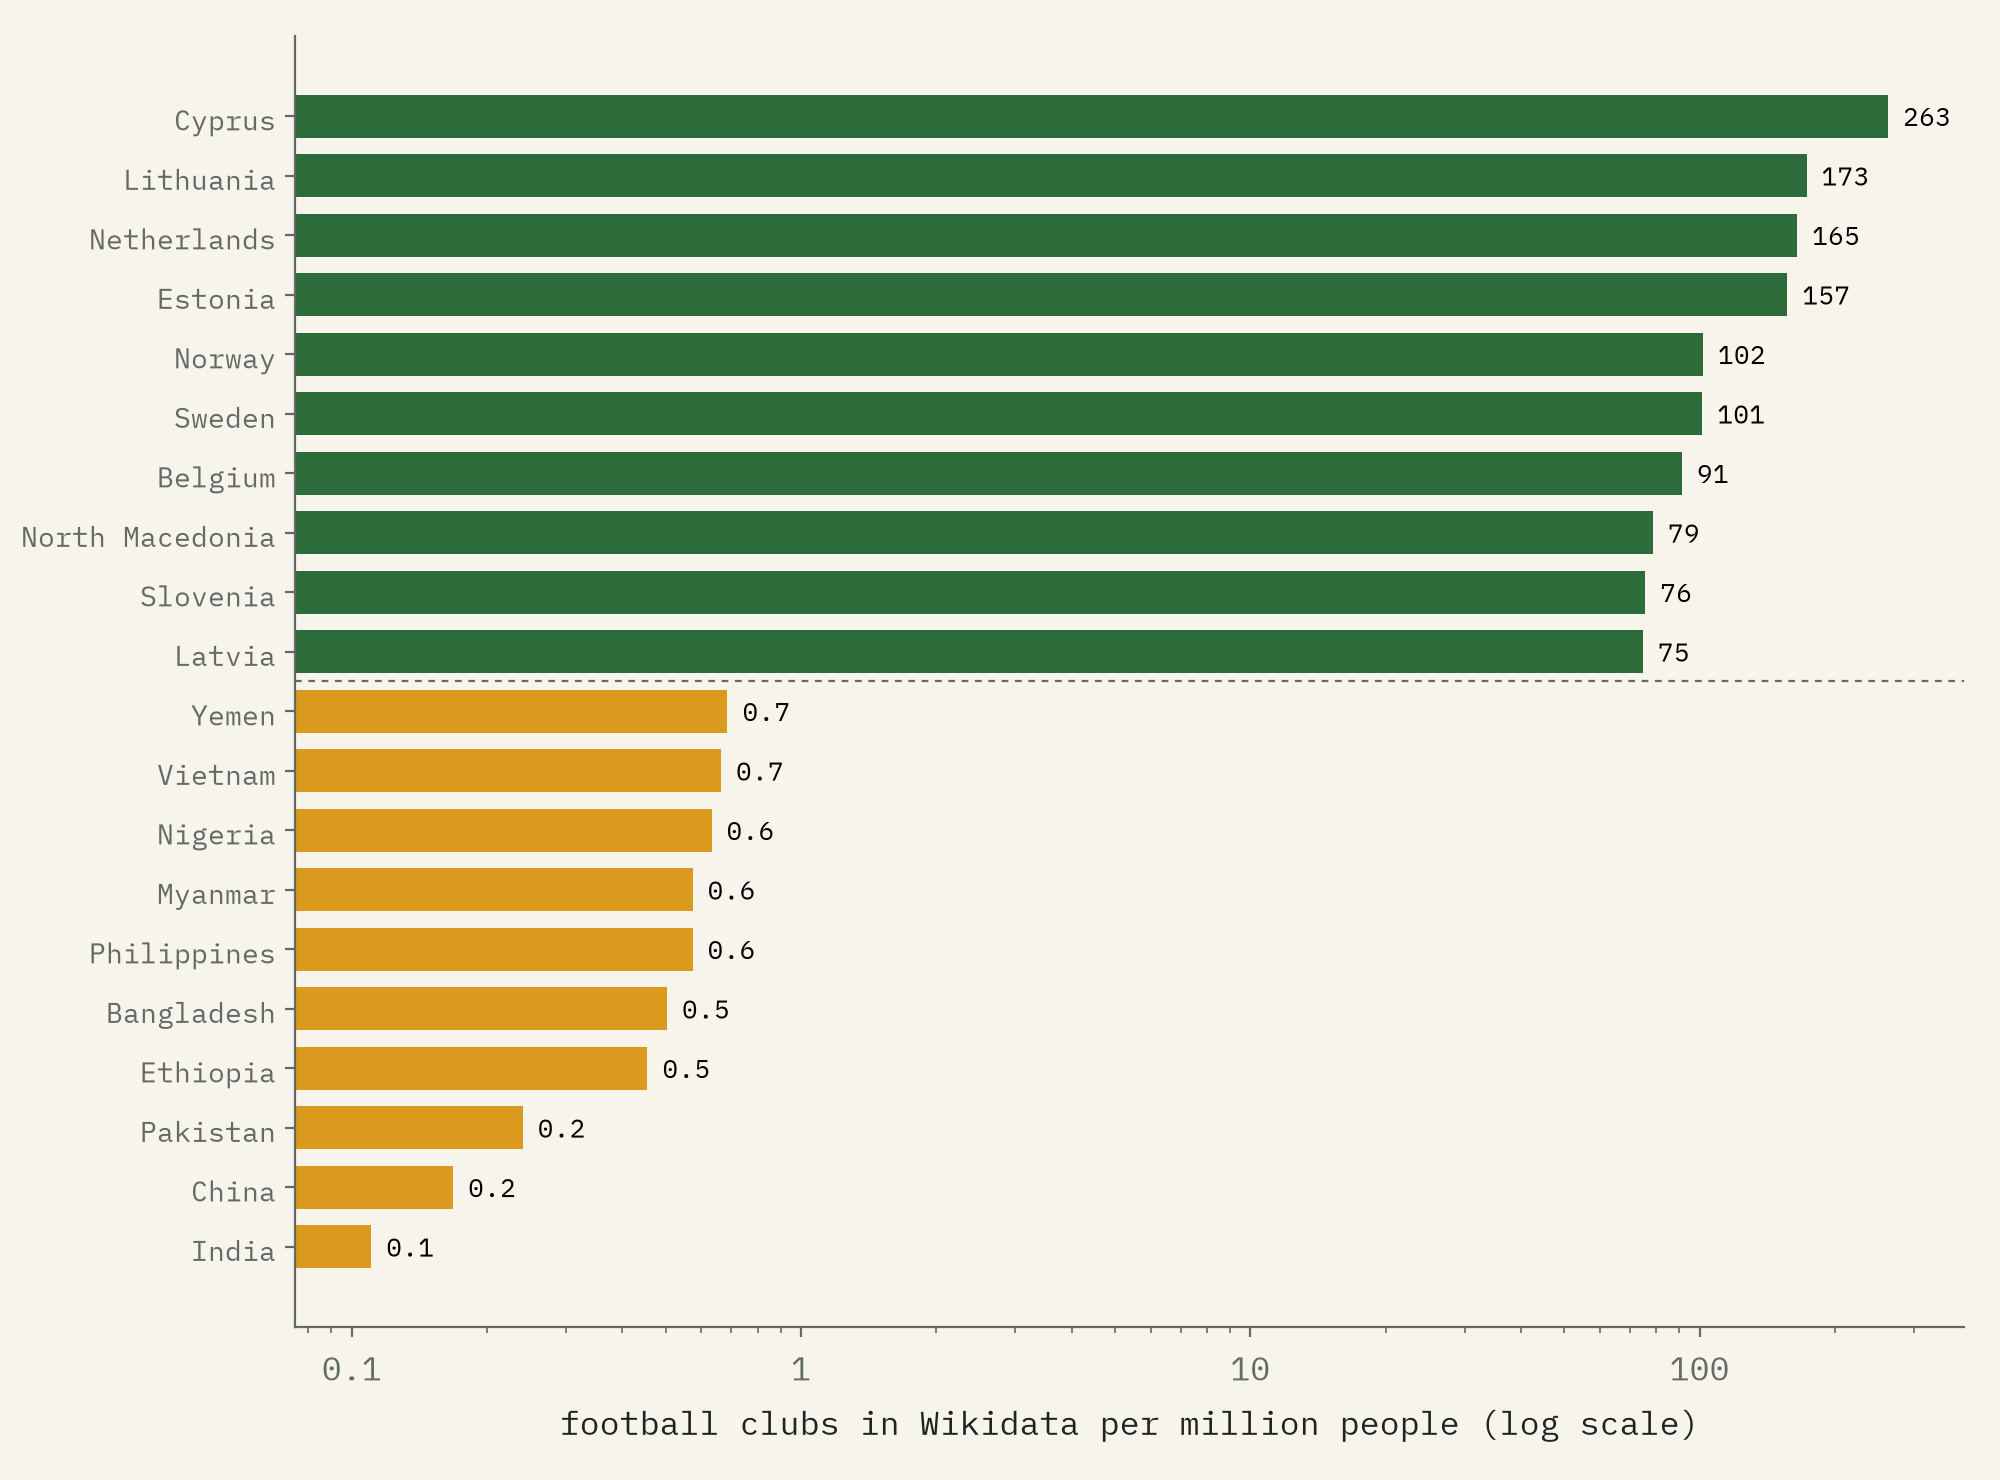
\includegraphics[width=.86\textwidth]{f_coverage.png}
\caption{Clubs in Wikidata per million people: the ten highest, and the ten lowest among countries of more than 20 million people.}\label{fig:cov}\end{figure}

\begin{table}[tbp]\centering\small\caption{Clubs by continent: share of clubs with a country, and the share of each continent's clubs with a founding year and with a point.}\label{tab:cov}\begin{tabular}{lrrrr}\toprule Continent & Clubs & Share & With a year & With a point\\\midrule
Europe & 25,560 & 60.8\% & 64\% & 32\%\\
South America & 3,403 & 8.1\% & 67\% & 50\%\\
North America & 2,989 & 7.1\% & 68\% & 59\%\\
Africa & 3,278 & 7.8\% & 50\% & 44\%\\
Asia & 6,002 & 14.3\% & 59\% & 44\%\\
Oceania & 800 & 1.9\% & 75\% & 47\%\\
\bottomrule\end{tabular}\end{table}

\section{Discussion}
The open record reproduces the broad history of football's spread that historians describe: a dense English and Scottish core in the 1860s and 1870s, early outposts along trade and imperial routes, a European boom after the First World War, and a long second wave across Africa, Asia and the Americas in the second half of the twentieth century. The diffusion front is clearly shaped by sea routes rather than distance, which fits accounts of football carried by merchants, sailors, engineers and teachers \citep{goldblatt}, though the data themselves say nothing about who those people were.

The stronger lesson is about the record. The Netherlands has more clubs in Wikidata than Germany, Cyprus more per head than anywhere, and India and China fewer per head than almost anywhere. Those are facts about Wikidata's editors, not about football. First-club years are more robust than counts, since they need only one well-documented old club, but even they depend on someone having entered that club with a date, and some first dates belong to older multi-sport societies.

\section{Limitations}
First, Wikidata is incomplete and uneven, and the totals count catalogued clubs, not clubs. Second, the definition of a club depends on Wikidata's classes, which mix clubs, teams and sections; my filters are name based and will both miss and wrongly remove some items. Third, a founding year may be that of a parent society, a refounding or a mistake, and dissolution dates are sparse and recent-heavy. Fourth, 3,177 points come from a town in the club's name and are approximate; others come from a club's current ground, which may have moved. Fifth, countries are present-day countries, so a club founded in the Austro-Hungarian empire is counted in today's Czech Republic or Ukraine. Sixth, nothing here identifies founders or their nationality. Finally, all counts are for one retrieval in 2026.

\section{Conclusion}
A single open query can trace football's spread from Sheffield to 222 countries and territories, show the waves of club founding by decade and continent, and record the clubs that died. It cannot say who founded them, and its gaps are themselves a finding. The atlas maps what is known, shows clearly where little is known, and lets readers explore both.

\section*{Data and code availability}
The interactive atlas is at \url{https://maps.tristanhotham.com/football-origins/}. Data and code are at \url{https://github.com/Tristan-Hotham/football-origins} and archived with this paper at \url{https://doi.org/10.5281/zenodo.23844505}. Derived data are released under CC BY 4.0 and code under the MIT licence.

\section*{AI statement}
I wrote the text, with drafting and editing assistance from Claude (Anthropic), which also helped prepare the analysis code. I reviewed and checked all text and results.

\begin{thebibliography}{9}
\bibitem[Bast and Buchhold(2017)]{qlever} Bast, H. and Buchhold, B. (2017) QLever: a query engine for efficient SPARQL+text search. \emph{Proceedings of the 2017 ACM Conference on Information and Knowledge Management}, 647 to 656. \url{https://qlever.cs.uni-freiburg.de/}
\bibitem[Curley(2016)]{engsoccer} Curley, J. P. (2016) engsoccerdata: English and European soccer results. R package, GPL-3. \url{https://github.com/jalapic/engsoccerdata}
\bibitem[Giulianotti and Robertson(2004)]{giulianotti} Giulianotti, R. and Robertson, R. (2004) The globalization of football: a study in the glocalization of the `serious life'. \emph{British Journal of Sociology}, 55(4), 545 to 568.
\bibitem[Goldblatt(2006)]{goldblatt} Goldblatt, D. (2006) \emph{The Ball is Round: A Global History of Football}. London: Viking.
\bibitem[Harvey(2005)]{harvey} Harvey, A. (2005) \emph{Football: The First Hundred Years. The Untold Story}. London: Routledge.
\bibitem[Natural Earth(2026)]{naturalearth} Natural Earth (2026) Admin 0 countries, admin 1 states and provinces, and populated places. Public domain. \url{https://www.naturalearthdata.com/}
\bibitem[Vrandečić and Krötzsch(2014)]{wikidata} Vrandečić, D. and Krötzsch, M. (2014) Wikidata: a free collaborative knowledgebase. \emph{Communications of the ACM}, 57(10), 78 to 85.
\end{thebibliography}
\end{document}
